\documentclass[11pt,a4paper]{article}

% ---------- Base packages ----------
\usepackage[T1]{fontenc}
\usepackage[utf8]{inputenc}
\IfFileExists{lmodern.sty}{\usepackage{lmodern}}{}
\usepackage{graphicx}
\usepackage{titlesec}
\usepackage{setspace}
\usepackage{geometry}
\geometry{margin=2.2cm}

\usepackage{subcaption}
\usepackage{float}
\usepackage{hyperref}

\usepackage{booktabs}
\usepackage{tabularx}
\usepackage{array}
\usepackage{enumitem}
\usepackage{xcolor}
\usepackage{listings}
\usepackage{caption}
\usepackage{amsmath}
\usepackage{tikz}
\usetikzlibrary{positioning,arrows.meta,shapes.geometric,fit,backgrounds,calc}

% ---------- Formatting ----------
\setstretch{1.05}
\emergencystretch=2em
\titleformat{\section}{\large\bfseries}{\thesection.}{1em}{}
\titleformat{\subsection}{\normalsize\bfseries}{\thesubsection.}{1em}{}
\hypersetup{colorlinks=true, linkcolor=blue, citecolor=blue, urlcolor=blue}

\captionsetup{font=small,labelfont=bf}
\setlist{itemsep=2pt,parsep=0pt,topsep=4pt}

\newcolumntype{L}[1]{>{\raggedright\arraybackslash}p{#1}}

% ---------- Code listing style ----------
\definecolor{lstbg}{gray}{0.96}
\lstdefinestyle{plain}{
  backgroundcolor=\color{lstbg},
  basicstyle=\ttfamily\scriptsize,
  breaklines=true,
  columns=fullflexible,
  frame=single,
  framesep=3pt,
  rulecolor=\color{gray!40},
  showstringspaces=false,
  xleftmargin=4pt,
  aboveskip=6pt,
  belowskip=6pt
}
\lstset{style=plain}

% ---------- Diagram colours (match the dashboard: amber = speed, teal = batch) ----------
\definecolor{speedc}{HTML}{D97706}
\definecolor{batchc}{HTML}{0F766E}
\definecolor{infrac}{HTML}{475569}
\definecolor{obsc}{HTML}{7C3AED}
\tikzset{
  box/.style={draw, rounded corners=2pt, align=center, font=\scriptsize,
              minimum height=0.95cm, text width=2.6cm, fill=white, line width=0.6pt},
  sbox/.style={box, draw=speedc, fill=speedc!8},
  bbox/.style={box, draw=batchc, fill=batchc!8},
  ibox/.style={box, draw=infrac, fill=infrac!6},
  obox/.style={box, draw=obsc, fill=obsc!7},
  arr/.style={-{Stealth[length=2.2mm]}, line width=0.6pt},
  sarr/.style={arr, draw=speedc},
  barr/.style={arr, draw=batchc},
  lbl/.style={font=\tiny, fill=white, inner sep=1pt},
}

% ---------- Screenshots ----------
% Screenshots live in docs/report/screenshots/. `.\scripts\voltstream.ps1 capture -Label <x>`
% and `faults -Capture` write most of them; the rest are taken by hand. Until a file exists
% the figure shows a labelled placeholder, so the document always compiles.
\newcommand{\figph}[2]{%
  \fbox{\begin{minipage}[c][#2][c]{0.90\textwidth}
    \centering\small\itshape #1
  \end{minipage}}%
}
\newcommand{\shot}[3]{%
  \IfFileExists{screenshots/#1.png}%
    {\includegraphics[width=\textwidth,height=#3,keepaspectratio]{screenshots/#1.png}}%
    {\figph{Screenshot: \texttt{screenshots/#1.png}\\[2pt] #2}{#3}}%
}

%----------------------------------------
\begin{document}

% --------- Cover Page ---------
\begin{titlepage}
    \centering
    \IfFileExists{Logo.jpeg}{\includegraphics[width=3cm]{Logo.jpeg}\par\vspace{1cm}}{\vspace*{2cm}}
    {\LARGE \textbf{Department of Electrical and Information Engineering}}\\[0.4cm]
    {\Large \textbf{University of Ruhuna}}\\[1.5cm]
    {\Large \textbf{Mini Project}}\\[0.2cm]
    {\large \textbf{Applied Big Data Engineering}}\\[0.2cm]
    {\large \textbf{EC8203}}\\[1.2cm]

    {\Large \textbf{Voltstream}}\\[0.3cm]
    {\large A Lambda-Architecture Data Platform for}\\[0.1cm]
    {\large Smart Grid Monitoring and Billing}\\[0.6cm]
    {\normalsize Use Case 3: Smart Grid Energy Monitoring \& Billing}\\[3cm]

    \begin{tabular}{rr}
        \large \textbf{EG/2021/4511} & \large \textbf{Fernando S.A.U.} \\
        \large \textbf{EG/2021/4516} & \large \textbf{Fonseka C. M.} \\
        \large \textbf{EG/2021/4525} & \large \textbf{} \\
    \end{tabular}\\[1cm]
    {\large \textbf{Computer Engineering (CE)}} \\[0.4cm]

    {\large \textbf{September 2026}}\\[1cm]
    {\small Repository: \url{https://github.com/Malee-Fonseka/voltstream}}

\end{titlepage}

% --------- Table of Contents ---------
\clearpage
\phantomsection
\addcontentsline{toc}{section}{Contents}
\tableofcontents
\clearpage

% =====================================================================
\section{Introduction and Use Case}
% =====================================================================

\subsection{Scope}

This report documents \textbf{voltstream}, an end-to-end data platform implementing
Use Case 3 of the module brief: \emph{Smart Grid Energy Monitoring and Billing}. The
system ingests continuous smart-meter telemetry and a once-daily tariff reference
feed, and serves a real-time zone dashboard alongside a daily per-household billing
report. It is built on a \textbf{Lambda architecture}; Section~\ref{sec:arch} sets out
that decision and the rejected Kappa alternative. Every number quoted in the Results
chapter was measured on the running system; none is a projection.

\subsection{Domain Problem}

Electricity cannot be meaningfully stored at grid scale, so supply must match demand
continuously. Distributed rooftop solar complicates this: it is generation the utility
neither controls nor dispatches, and cloud cover crossing a zone can cut contribution
substantially within a minute, leaving a shortfall that must be absorbed by plant
requiring minutes to ramp. \emph{Renewable contribution by zone, right now} is
therefore an operational signal that triggers a physical control action, and it is
worthless if it arrives late.

In parallel, a separate department bills the same households from the same readings.
Billing is not consumption multiplied by a rate. It combines block tariffs with
block-dependent rates, tier-dependent fixed charges, subsidy discounts, and net
metering that credits exported solar against imported grid energy.

\subsection{Interpreted Business Requirements}

The brief's business question has two halves---\emph{what is the current grid load and
renewable contribution by zone}, and \emph{what will each household's bill look like
once daily tariff data is applied}---and they belong to two consumers whose requirements
are in direct opposition. Table~\ref{tab:twoconsumers} is the origin of the architecture
decision that follows.

\begin{table}[H]
\centering
\caption{The two consumers have opposing requirements.}
\label{tab:twoconsumers}
\small
\begin{tabularx}{\textwidth}{L{3.1cm} X X}
\toprule
\textbf{Dimension} & \textbf{Grid operations} & \textbf{Billing} \\
\midrule
Question & Grid load and renewable mix by zone & Household bill once daily tariff is applied \\
Latency & Seconds & End of simulated day \\
A 2\% error & Harmless; does not change a ramping decision & Legally actionable \\
Yesterday's answer & Disposable & Reproducible for years \\
Late data & May be ignored & Must be included \\
Restatement & Never & Months later, on demand \\
Auditability & Not required & Full lineage to source readings \\
\bottomrule
\end{tabularx}
\end{table}

The second question's phrasing---\emph{once daily tariff data is applied}---encodes a
dependency on data that does not exist until the day closes. No streaming technique
removes that dependency, because it is a property of the business process rather than
of the technology.

The brief's three suggested outputs map directly onto delivered components:
\begin{itemize}
  \item \emph{API endpoint for real-time grid load and renewable mix by zone} ---
        \texttt{GET /api/v1/zones/load} and \texttt{/zones/history}, and the
        dashboard's Live grid tab (Section~\ref{sec:res-live}).
  \item \emph{Threshold-based alert when renewable contribution is low} ---
        the \texttt{LowRenewableContribution} Prometheus rule, plus four further
        pipeline-health rules (Section~\ref{sec:alerts}).
  \item \emph{Daily consolidated billing and solar-contribution report per household} ---
        the batch layer's bills, served through the merge endpoint, the dashboard's
        Household bills and Daily report tabs, and a Markdown report file written to
        object storage for every closed day (Section~\ref{sec:res-report}).
\end{itemize}

% =====================================================================
\section{Requirements}
% =====================================================================

\subsection{Functional}

\begin{enumerate}[label=\textbf{F\arabic*.},leftmargin=2.2em,itemsep=1pt]
  \item Ingest continuous smart-meter readings, and one tariff reference file (plus
        a weather forecast file) per simulated day.
  \item Retain every raw event immutably for unbounded reprocessing.
  \item Compute and expose per-zone load and renewable contribution over event-time
        windows.
  \item Compute per-household daily bills applying solar netting, block tariffs,
        fixed charges, subsidy discounts and export credit.
  \item Serve a live dashboard, a consolidated daily report, and threshold-based
        alerts including low renewable contribution.
\end{enumerate}

\subsection{Non-Functional}

\begin{table}[H]
\centering
\caption{Non-functional requirements, their justification, and the measured outcome
(Section~\ref{sec:results}).}
\label{tab:nfr}
\small
\begin{tabularx}{\textwidth}{L{0.7cm} L{4.2cm} L{4.0cm} X}
\toprule
\textbf{ID} & \textbf{Requirement} & \textbf{Rationale} & \textbf{Measured} \\
\midrule
N1 & Speed-layer latency below 60\,s & Grid ramping decision window & Mean 6.3\,s; 0 of $\sim$2{,}300 over 60\,s \\
N2 & Batch complete within 10 real minutes of day close & Demonstration tractability & Whole DAG 59\,s after a 90\,s grace \\
N3 & Zero data loss on single-component failure & Bus retention plus immutable master dataset & 0 lost after SIGKILL of archiver and of speed layer \\
N4 & Unbounded restatement horizon & Dispute window exceeds bus retention & Day restated from Parquet; history kept \\
N5 & Reproducible from a clean clone & Assessment requirement & One command; \texttt{make cold-start} rebuilds from a fresh clone \\
N6 & Every pipeline stage observable & Failures must be detectable & 8 metrics, 5 alert rules, 3 dashboards \\
\bottomrule
\end{tabularx}
\end{table}

\subsection{Simulated Clock}
\label{sec:simclock}

Simulated time is compressed so the pipeline is demonstrable within a session:
\[
  1 \text{ simulated day} = 5 \text{ real minutes}, \qquad \mathrm{TIME\_SCALE} = 288
\]
Simulated time begins at 2026-01-01 00:00 UTC at the instant the stack is started
(the anchor \texttt{VOLTSTREAM\_ANCHOR\_REAL} is stamped into \texttt{.env}); day 1 is
therefore partial and 2026-01-02 is the first complete day. With a 2-second emit
interval each meter produces 150 readings per simulated day on a fixed tick grid.
Across 50 households in 5 grid zones this yields approximately 7{,}500 raw events,
480 zone-window rows and 50 bill rows per simulated day. One 15-simulated-minute window
lasts 3.125 real seconds.

All timestamps and all windowing operate on \emph{simulated} time; only latency
metrics use wall-clock time (measured from the Kafka record timestamp, never from
\texttt{event\_ts}). A single module, \texttt{simclock.py}, performs the conversion, and
every duration in \texttt{config/base.yaml} carries an explicit \texttt{\_sim\_minutes}
or \texttt{\_real\_seconds} suffix, so no component computes simulated time
independently or ambiguously.

% =====================================================================
\section{Architecture Decision: Lambda versus Kappa}
\label{sec:arch}
% =====================================================================

\subsection{The Two Candidates}

\textbf{Lambda} \cite{marz} maintains two processing paths over one immutable input: a
batch layer recomputing authoritative results from all history, a speed layer computing
approximate results from recent data, and a serving layer merging them, so that
$\mathit{query} = \mathit{merge}(\mathit{batch\_view}, \mathit{realtime\_view})$.

\textbf{Kappa} \cite{kreps} maintains a single path. Everything is a stream, and
correction is achieved by replaying the log from an earlier offset through the same code.

\subsection{Decision and Evaluation}

\textbf{Lambda is selected.} The decision follows from Table~\ref{tab:twoconsumers},
evaluated against the four criteria the assessment identifies as decisive.

\begin{table}[H]
\centering
\caption{Architecture evaluation. Replay and consistency are the decisive criteria.}
\label{tab:archeval}
\small
\begin{tabularx}{\textwidth}{L{1.9cm} X L{1.9cm}}
\toprule
\textbf{Criterion} & \textbf{Analysis} & \textbf{Verdict} \\
\midrule
Latency &
Two consumers separated by roughly two orders of magnitude: seconds for operations,
hours for billing. A single path must be tuned for one, penalising the other. Tuning
for exactness through long watermarks and complete-day state makes the operations view
unusably late; tuning for latency makes billing incorrect. &
Lambda \\
\addlinespace
Replay &
Billing disputes and retroactive tariff corrections carry a restatement horizon of
\emph{months}. Practical Kafka retention is \emph{days}. Kappa's correction
mechanism---replay from an earlier offset---is unavailable beyond retention. Lambda's
batch layer replays from object storage, which is unbounded. &
Lambda \\
\addlinespace
Cost &
Lambda pays for two codepaths and a nightly compute burst. Kappa pays for either
extended retention or very large long-lived state holding per-household billing
accumulators across the horizon. Both are affordable at our volume, but Kappa's state
cost grows with $\mathit{households} \times \mathit{horizon}$, the worse curve. &
Lambda, narrowly \\
\addlinespace
Consistency &
Billing requires an immutable, auditable ledger independent of the message bus, with
lineage from final amount back to source readings. Lambda's master dataset provides
this. Kappa's ground truth is the log itself---a transport system governed by a
retention policy, an uncomfortable foundation for a financial audit trail. &
Lambda, decisively \\
\bottomrule
\end{tabularx}
\end{table}

\subsection{The Rejected Alternative: Kappa}

Kappa is a genuinely viable design here and is presented as such.

\paragraph{How it would work.} Tariff data would be a \emph{compacted} Kafka
topic keyed on household, retaining the latest tariff per household. A single
Structured Streaming job would perform a stream--table join against meter readings.
Corrections would be made by deploying fixed code, replaying from an earlier offset
into a new output table, and atomically switching readers to it.

\paragraph{Its genuine advantages.} One codebase, eliminating any possibility of
speed--batch divergence---Lambda's canonical weakness. Operational simplicity: one job
to deploy and monitor rather than two plus an orchestrator. Conceptual cleanliness:
batch is simply a bounded stream, with no second mental model to maintain.

\paragraph{Grounds for rejection.}
\begin{enumerate}[itemsep=2pt]
  \item \textbf{Retention horizon mismatch.} Decisive. Billing restatement must remain
        possible months later, while retention is measured in days. Kappa's correction
        mechanism is unavailable at precisely the point billing most requires it.
  \item \textbf{Audit independence.} Finance requires a ledger that does not depend on
        the configuration of the message bus. A retention-policy change should not be
        capable of destroying a billing audit trail.
  \item \textbf{State cost and fragility.} Holding per-household tiered billing
        accumulators as streaming state across a months-long horizon is expensive and
        fragile compared with a bounded nightly job over a fixed partition.
\end{enumerate}

\subsection{Lambda's Cost and Our Structural Mitigation}
\label{sec:drift}

Lambda's cost is real: the same business logic exists in two codepaths and can
silently diverge. Concretely, if the speed layer treats the first tariff block as
ending at 60\,kWh while the batch layer treats it as ending at 61\,kWh, a household
consuming near that boundary sees one figure during the day and a different figure on
the final bill. The defect is invisible unless the boundary is specifically exercised.

Our mitigation is structural rather than procedural:

\begin{enumerate}[itemsep=3pt]
  \item \textbf{A shared pure module.} \texttt{voltstream/core/} holds netting, tariff,
        money-rounding, key-derivation and validation logic as pure functions with no
        I/O, no clock access and no database calls. Both the streaming and batch jobs
        import it. It is a \emph{peer} of the layer packages rather than nested inside
        either, so the sharing is visible in the repository structure itself. CI enforces
        100\% line coverage on it.
  \item \textbf{A consistency test pinning the implementations together.}
        \texttt{core/tariff.py} holds scalar \texttt{Decimal} functions;
        \texttt{core/spark\_expr.py} holds the same logic as Spark \texttt{Column}
        expressions. This duplication is necessary---the API container has no Spark
        runtime, while the Spark path must use Column expressions rather than
        user-defined functions to preserve query optimisation and avoid per-row
        serialisation. \texttt{tests/consistency/test\_pure\_vs\_spark.py} generates
        5{,}000 random inputs, executes both implementations, and asserts identical
        output to the cent. It additionally sweeps each tariff block boundary in
        hundredth-kWh steps and includes half-cent rounding ties, because an off-by-one at
        a boundary is precisely the defect uniform random sampling is least likely to find.
\end{enumerate}

Divergence in \emph{logic} between the layers is therefore a test failure rather than a
matter of developer discipline. Divergence in \emph{inputs}---a stale tariff, dropped late
readings---is intended, and is measured at run time (Section~\ref{sec:res-recon}).

\subsection{Contingency: What Would Reverse This Decision}
\label{sec:contingency}

The choice of Lambda is contingent on one constraint: \textbf{the master dataset must
outlive the message bus's retention window}. Adopting Kafka tiered storage, which
offloads old segments to object storage, or a table format such as Apache Iceberg or
Delta Lake, which grants the log ACID semantics and unbounded queryable history,
removes that constraint. At that point Kappa's single codebase becomes the better
trade and migration would be justified. Stating the condition under which the decision
reverses is, in our view, a stronger position than defending Lambda unconditionally.

% =====================================================================
\section{Solution Architecture}
\label{sec:solution}
% =====================================================================

\begin{figure}[H]
\centering
\resizebox{\textwidth}{!}{%
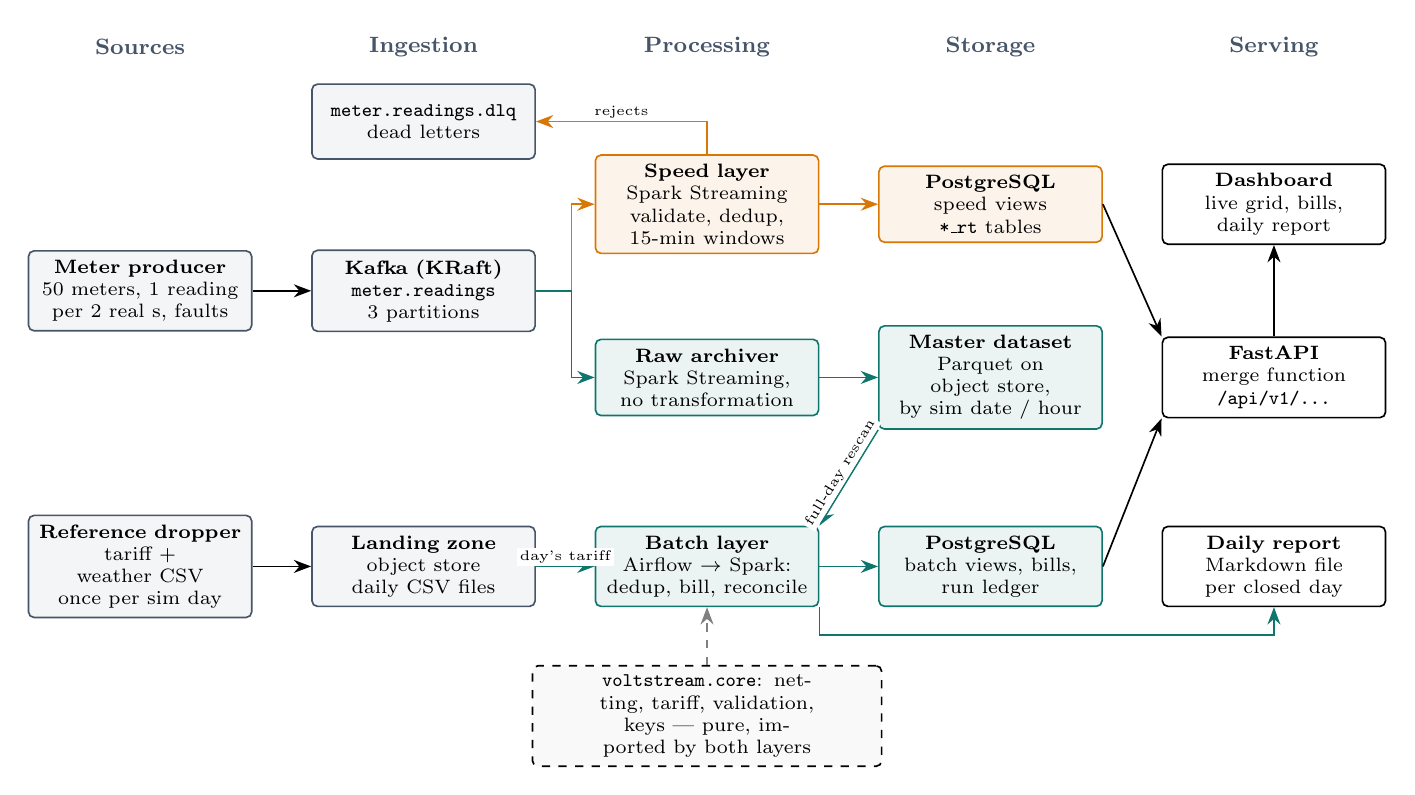
\begin{tikzpicture}
  \foreach \x/\t in {0/Sources, 3.6/Ingestion, 7.2/Processing, 10.8/Storage, 14.4/Serving}
    \node[font=\footnotesize\bfseries, text=infrac] at (\x,5.4) {\t};

  \node[ibox] (prod) at (0,2.3) {\textbf{Meter producer}\\50 meters, 1 reading\\per 2 real s, faults};
  \node[ibox] (drop) at (0,-1.2) {\textbf{Reference dropper}\\tariff + weather CSV\\once per sim day};

  \node[ibox] (dlq) at (3.6,4.45) {\texttt{meter.readings.dlq}\\dead letters};
  \node[ibox] (kafka) at (3.6,2.3) {\textbf{Kafka (KRaft)}\\\texttt{meter.readings}\\3 partitions};
  \node[ibox] (land) at (3.6,-1.2) {\textbf{Landing zone}\\object store\\daily CSV files};

  \node[sbox] (speed) at (7.2,3.4) {\textbf{Speed layer}\\Spark Streaming\\validate, dedup,\\15-min windows};
  \node[bbox] (arch) at (7.2,1.2) {\textbf{Raw archiver}\\Spark Streaming,\\no transformation};
  \node[bbox] (batch) at (7.2,-1.2) {\textbf{Batch layer}\\Airflow $\rightarrow$ Spark:\\dedup, bill, reconcile};

  \node[sbox] (pgs) at (10.8,3.4) {\textbf{PostgreSQL}\\speed views\\\texttt{*\_rt} tables};
  \node[bbox] (master) at (10.8,1.2) {\textbf{Master dataset}\\Parquet on\\object store,\\by sim date / hour};
  \node[bbox] (pgb) at (10.8,-1.2) {\textbf{PostgreSQL}\\batch views, bills,\\run ledger};

  \node[box] (dash) at (14.4,3.4) {\textbf{Dashboard}\\live grid, bills,\\daily report};
  \node[box] (api) at (14.4,1.2) {\textbf{FastAPI}\\merge function\\\texttt{/api/v1/\dots}};
  \node[box] (rep) at (14.4,-1.2) {\textbf{Daily report}\\Markdown file\\per closed day};

  \node[box, dashed, text width=4.2cm, fill=gray!5] (core) at (7.2,-3.1)
      {\texttt{voltstream.core}: netting, tariff, validation,\\keys --- pure, imported by both layers};

  \draw[arr] (prod) -- (kafka);
  \draw[arr] (drop) -- (land);
  \draw[sarr] (kafka.east) -- ++(0.45,0) |- (speed.west);
  \draw[barr] (kafka.east) -- ++(0.45,0) |- (arch.west);
  \draw[sarr] (speed.north) |- node[lbl, pos=0.75, above]{rejects} (dlq.east);
  \draw[barr] (arch) -- (master);
  \draw[barr] (master.south west) -- node[lbl, sloped, above]{full-day rescan} (batch.north east);
  \draw[barr] (land) -- node[lbl, above]{day's tariff} (batch);
  \draw[sarr] (speed) -- (pgs);
  \draw[barr] (batch) -- (pgb);
  \draw[arr] (pgs.east) -- (api.north west);
  \draw[arr] (pgb.east) -- (api.south west);
  \draw[arr] (api) -- (dash);
  \draw[barr] (batch.south east) -- ++(0,-0.35) -| (rep.south);
  \draw[arr, dashed, gray] (core) -- (batch);
\end{tikzpicture}}
\caption{End-to-end architecture across ingestion, processing, storage and serving.
Amber is the speed path (process, then store); teal is the batch path (store, then
process). Both consume the same Kafka topic independently, each with its own checkpointed
offsets. The dashed \texttt{core} module is imported by both processing layers.}
\label{fig:lambda}
\end{figure}

\subsection{The Three Views}

\paragraph{Master dataset.} Every raw event, unmodified, written as Parquet to object
storage and partitioned by simulated date and hour; each day's tariff file is archived
alongside once billed. Nothing is updated in place. This is the ground truth from which
the batch layer recomputes, and it is what makes replay possible after bus retention
expires. The archiver performs no validation or filtering on purpose: filtering there
would destroy the bug-recovery property that justifies the dataset's existence.

\paragraph{Speed view.} Event-time tumbling windows of 15 simulated minutes per zone,
producing total consumption, total solar generation, renewable ratio and active meter
count. A per-household running total for the current simulated day is also maintained,
costed against \emph{yesterday's} tariff---deliberately stale and labelled provisional,
because today's tariff does not yet exist.

\paragraph{Batch view.} Triggered by the arrival of a day's tariff file. Reads the
complete day's partition, validates and deduplicates, joins the day's own tariff, applies
netting and block-tariff logic from \texttt{core/}, writes finalised bills, rolls up exact
daily zone totals, reconciles against the speed view, publishes the daily report, and marks
the day closed in the run ledger.

\subsection{The Merge Function}
\label{sec:merge}

\begin{lstlisting}[caption={Serving-layer merge logic (\texttt{api/routers/households.py}).},label={lst:merge}]
GET /api/v1/households/{id}/bill?date=YYYY-MM-DD

    if pipeline_runs has a successful batch_billing run for this sim_date:
        return household_bill_daily row,  source="batch", provisional=false
    else:
        return household_running_rt row,  source="speed", provisional=true
\end{lstlisting}

The batch view wins unconditionally because it is strictly better informed: it
observed the late events the speed layer discarded past its watermark, applied the
correct day's tariff rather than a stale one, and executed deterministically over a
closed input set. There is no case in which the speed estimate is more correct. The
response always reports which view served it and which day's tariff priced it, making
the provisional-to-final transition observable from the API itself.

\begin{figure}[H]
\centering
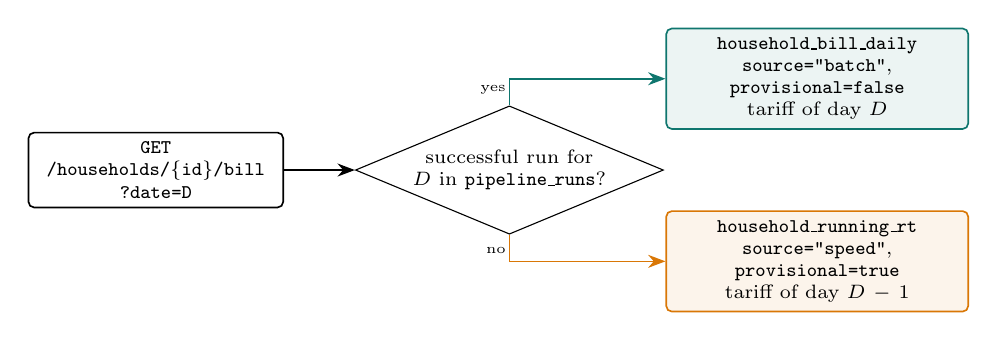
\begin{tikzpicture}[node distance=0.5cm and 0.9cm]
  \node[box, text width=3.0cm] (req) {\texttt{GET /households/\{id\}/bill}\\\texttt{?date=D}};
  \node[draw, diamond, aspect=2.4, align=center, font=\scriptsize, inner sep=1pt, right=of req] (dec)
       {successful run for\\$D$ in \texttt{pipeline\_runs}?};
  \node[bbox, text width=3.6cm, above right=0.1cm and 1.0cm of dec] (b)
       {\texttt{household\_bill\_daily}\\\texttt{source="batch"}, \texttt{provisional=false}\\tariff of day $D$};
  \node[sbox, text width=3.6cm, below right=0.1cm and 1.0cm of dec] (s)
       {\texttt{household\_running\_rt}\\\texttt{source="speed"}, \texttt{provisional=true}\\tariff of day $D-1$};
  \draw[arr] (req) -- (dec);
  \draw[barr] (dec.north) |- node[lbl, pos=0.3, left]{yes} (b.west);
  \draw[sarr] (dec.south) |- node[lbl, pos=0.3, left]{no} (s.west);
\end{tikzpicture}
\caption{The merge function: the architecture rendered as product behaviour.}
\label{fig:merge}
\end{figure}

\subsection{Domain Modelling Decisions}

\paragraph{Event time, not processing time.} Readings carry their own
\texttt{event\_ts} and arrive out of order due to network buffering. All windowing
uses event time with a watermark. Windowing on arrival time would let a network delay
silently relocate a reading into the wrong window, after which daily totals would
cease to reconcile.

\paragraph{Solar netting.} The non-trivial transformation, applied before tariff
evaluation (\texttt{core/netting.py}):
\begin{align}
  \mathit{self\_consumed}   &= \min(\mathit{solar},\ \mathit{consumption}) \\
  \mathit{billable\_import} &= \mathit{consumption} - \mathit{self\_consumed} \\
  \mathit{export}           &= \mathit{solar} - \mathit{self\_consumed}
\end{align}
$\mathit{billable\_import}$ is charged block by block against the tariff, then
\begin{equation}
  \mathit{total} = \mathit{energy\_charge} + \mathit{fixed\_charge}
                 - \mathit{subsidy\_discount} - \mathit{export\_credit},
\end{equation}
with money rounded half-up to two decimal places at pinned points only
(\texttt{core/money.py}), identically in both layers.

\paragraph{Idempotency and partitioning.} Kafka provides at-least-once delivery; the
deduplication key is $(\mathit{meter\_id}, \mathit{event\_ts})$, defined once in
\texttt{core/keys.py} and used by both layers. The Kafka \emph{message key} is
\texttt{household\_id}, achieving two objectives at once: per-household ordering within
a partition, and co-partitioning with the tariff join key.

% =====================================================================
\section{Technology Stack and Justification}
\label{sec:stack}
% =====================================================================

Selections are justified against use-case constraints rather than general popularity.
Each entry names the alternative rejected and the reason.

\begin{table}[H]
\centering
\caption{Technology selections and the constraint each satisfies.}
\label{tab:stack}
\small
\begin{tabularx}{\textwidth}{L{2.0cm} L{2.4cm} X L{2.2cm}}
\toprule
\textbf{Layer} & \textbf{Selected} & \textbf{Constraint satisfied} & \textbf{Rejected} \\
\midrule
Ingestion & Apache Kafka 3 (KRaft) & A replayable log is a precondition for Lambda; independent
multi-consumer reads enable the two-branch fan-out & RabbitMQ; direct DB writes \\
\addlinespace
Stream \& batch processing & Spark 3.5 Structured Streaming and batch & One API for both
layers enables the shared \texttt{core/} module; native event-time watermarking & Storm; Flink \\
\addlinespace
Master dataset & Parquet on S3-compatible object store & Columnar, compressed, immutable;
partition-pruned full-day rescans; retention decoupled from compute & HDFS; raw CSV/JSON \\
\addlinespace
Serving store & PostgreSQL 16 & Relational joins, ACID for financial writes, indexed
point lookups; post-aggregation write volume is trivial & Cassandra; MongoDB \\
\addlinespace
Orchestration & Apache Airflow 3 & Sensors, retries, run history and re-runnable,
per-date billing runs---the restatement mechanism itself & cron \\
\addlinespace
Observability & Prometheus, Alertmanager, Grafana & Pull scraping suits containers;
alert rules are declarative, version-controlled and unit-tested & Bespoke log parsing \\
\addlinespace
Serving API & FastAPI & Async, generated OpenAPI docs, schema enforcement at the
boundary & Flask \\
\addlinespace
Deployment & Docker Compose & One-command reproducible stack for graders, no cloud
account & Kubernetes \\
\bottomrule
\end{tabularx}
\end{table}

\subsection{Ingestion: Apache Kafka}

Kafka is an append-only log rather than a queue: reading does not delete, and
consumers track their own offsets. Three capabilities follow, all load-bearing here.
\textbf{Replay}---a speed-layer defect is corrected by resetting the offset and
reprocessing. \textbf{Decoupling}---the producer is indifferent to consumer
availability, so Kafka absorbs bursts and outages. \textbf{Independent multi-consumer
reads}---the speed layer and raw archiver read the same topic with entirely separate
offsets, which is what makes the two-branch Lambda shape possible from a single source.

\paragraph{Where those offsets actually live.} Not in Kafka. Spark Structured Streaming
\emph{assigns} partitions directly rather than subscribing as a consumer group, and
commits its offsets to its own checkpoint. A consequence worth stating plainly, because
it contradicts the usual description of Kafka fan-out: \texttt{kafka-consumer-groups
-{}-list} shows nothing for either branch, and setting \texttt{kafka.group.id} does not
change that. We verified this directly. The independence is real and was measured; it is
simply visible in the checkpoints rather than in Kafka's group metadata. During the
restart test the archiver had committed 73 micro-batches while the speed layer's queries
sat at 8--9, each advancing at its own rate, and killing one left the other untouched.

Three partitions are configured, bounding consumer parallelism. Default retention of
approximately seven days is the mechanical fact underlying Section~\ref{sec:arch}.
KRaft mode removes ZooKeeper, one container fewer for the same guarantees.

\paragraph{Rejected.} RabbitMQ removes messages on acknowledgement, eliminating both
replay and independent multi-consumer reading. Writing directly to the database
forfeits buffering, backpressure and replay, and couples producer availability to
database availability.

\subsection{Stream Processing: Spark Structured Streaming}

Because the batch and streaming APIs are identical, the billing logic resides in one
shared module imported by both jobs (Section~\ref{sec:drift}). Lambda's canonical
weakness is not mitigated rhetorically---the class of defect is structurally
eliminated. No other candidate engine offers this property as directly.

A watermark encodes the system's belief about maximum lateness. The trade-off is
explicit: a shorter watermark gives lower latency but discards more late data; a
longer one gives more complete results at higher latency and greater retained state.
The speed layer chooses low latency and accepts discarding stragglers; the batch layer
requires no watermark at all, because it rescans a closed day. That divergence is not
an inconsistency---it is each layer tuned for its own consumer, which is the benefit
Lambda exists to provide.

\paragraph{Rejected: Storm.} Attains genuinely lower latency, in the single-digit
millisecond range, but provides no native event-time windowing or watermarks and no
batch API for code sharing. Our latency requirement is seconds, so Storm's sole
advantage is irrelevant here while both its costs are real.

\paragraph{Rejected: Flink.} In our assessment the superior pure streaming engine,
with true event-at-a-time processing and a stronger state backend. It is rejected on
grounds specific to this project rather than on technical merit: no unified batch story
in the same Python idiom for code sharing, a steeper learning curve within a two-week
budget, and a latency requirement Spark already satisfies comfortably (measured mean
6.3\,s against a 60\,s budget).

\subsection{Master Dataset: Parquet on Object Storage}

\paragraph{Why a master dataset is required.} Lambda's premise is
$\mathit{query} = f(\mathit{all\ data})$, which cannot be computed if the data was
discarded. Concretely: a tier-boundary comparison using \texttt{>} instead of
\texttt{>=} renders every boundary-adjacent bill incorrect, and with raw inputs
retained the function is fixed and the range restated---without them, the incorrect
answer is the only answer that exists. More generally, \emph{raw data is a superset of
every aggregate that might later be required; an aggregate is a superset of nothing}.
Re-executing yesterday's job over yesterday's partition produces identical output, and
that determinism constitutes the audit guarantee (demonstrated in
Section~\ref{sec:res-restate}).

\paragraph{Why Parquet.} Columnar layout yields four benefits over row-oriented CSV or
JSON: \emph{column pruning} (billing reads a handful of columns from a wider schema),
\emph{effective compression} (\texttt{grid\_zone}, with five distinct values, is
dictionary-encoded), \emph{embedded schema and real types} (\texttt{event\_ts} is a
genuine timestamp rather than a re-inferred string), and \emph{predicate pushdown}.
Partitioning by simulated date and hour compounds this: the daily job's directory
listing alone excludes every other day.

\paragraph{Why a local S3-compatible store rather than AWS S3.} Object storage decouples
storage from compute. The code speaks only the S3 API through \texttt{s3a://} paths, so
migration to AWS is a change of endpoint and credentials. A local store is preferred
because reproducibility is an assessment requirement: a grader runs one command with no
cloud account and no network dependency. MinIO withdrew its community images during the
project, so the stack runs \texttt{pgsty/silo}, a MinIO-compatible fork pinned to a release
tag (decision D8); because only the S3 API is used, replacing it is configuration, not
code. HDFS was rejected: its NameNode overhead is unjustified at this scale and it
reintroduces the compute--storage coupling object storage removes.

\subsection{Serving Store: PostgreSQL}

The serving layer is optimised for the read pattern, not for ingestion. Our patterns
are point lookups by $(\mathit{household\_id}, \mathit{sim\_date})$, aggregation over
recent windows grouped by zone, and joins between billing, ledger and household
rows---small result sets of relational shape. PostgreSQL supplies joins, ACID
transactions (a billing run lands entirely or not at all), \texttt{JSONB} for the
per-block breakdown, and \texttt{ON CONFLICT DO UPDATE} for idempotent upserts from
micro-batches that may be replayed. Measured API reads are 8.7--14.7\,ms at the median.

\paragraph{Rejected: Cassandra.} Excellent at high write throughput at scale, but
queries are restricted to the partition key, joins and ad-hoc aggregation are
unavailable, and consistency is eventual. Our post-aggregation write volume is a few
hundred rows per simulated day; selecting Cassandra would optimise for a problem this
system does not have.

\subsection{Orchestration: Apache Airflow}

Airflow supplies a dependency graph, sensors, retries with backoff and a persistent run
history. One design problem is specific to simulated time: Airflow schedules on
\emph{real} time and addresses runs by data interval, so no cron expression can express
``once per simulated day''. The solution is a \texttt{tariff\_watcher} DAG that polls the
landing zone every real minute and triggers \texttt{daily\_billing} once per tariff file,
with a run id derived from the file's date (\texttt{billing\_\_2026-01-02}). This is
idempotent by construction: re-listing the same file yields the same run id, which Airflow
skips. A restatement is simply a further run for the same date (\texttt{\dots\_\_r1}),
which is how the architecture's correction mechanism becomes executable rather than
described.

The DAGs are deliberately thin: they start Spark jobs in their own containers (through a
Docker socket proxy, never the raw socket) and verify results, containing no business
logic. The Airflow image contains no project code at all, isolating Airflow's constrained
dependency set from PySpark and FastAPI. Cron was rejected as it offers no dependency graph,
no retry semantics, no run history and no re-run by date. Batch SLA monitoring is done in
Prometheus (\texttt{BatchSLAMiss}) rather than with Airflow SLAs, which Airflow 3 removed.

\subsection{Observability: Prometheus, Alertmanager, Grafana}

Prometheus scrapes a \texttt{/metrics} endpoint on each long-running service, a pull model
that suits containers because services need only expose an endpoint. Batch containers exit
before a scrape could reach them, so they push to a Pushgateway on exit. Metrics are
labelled time series, so one metric labelled by zone supports per-zone slicing.
Alertmanager consumes rules from a repository file, making alerting version-controlled,
reviewable and unit-testable with \texttt{promtool}. Grafana is provisioned from files, so
all three dashboards exist on a fresh start with no manual steps.

% =====================================================================
\section{Implementation}
\label{sec:implementation}
% =====================================================================

\subsection{Deployment Topology}

Eighteen containers are arranged in four dependency tiers under Docker Compose with
health-condition dependencies (Figure~\ref{fig:deployment}). The tier-2 bootstrap
containers execute once and exit; without them, tier-3 services start correctly but fail
on first write. The whole stack is started, health-checked and verified with one command
(\texttt{.\textbackslash scripts\textbackslash voltstream.ps1 run} on Windows,
\texttt{make up} on Linux).

\begin{figure}[H]
\centering
\resizebox{\textwidth}{!}{%
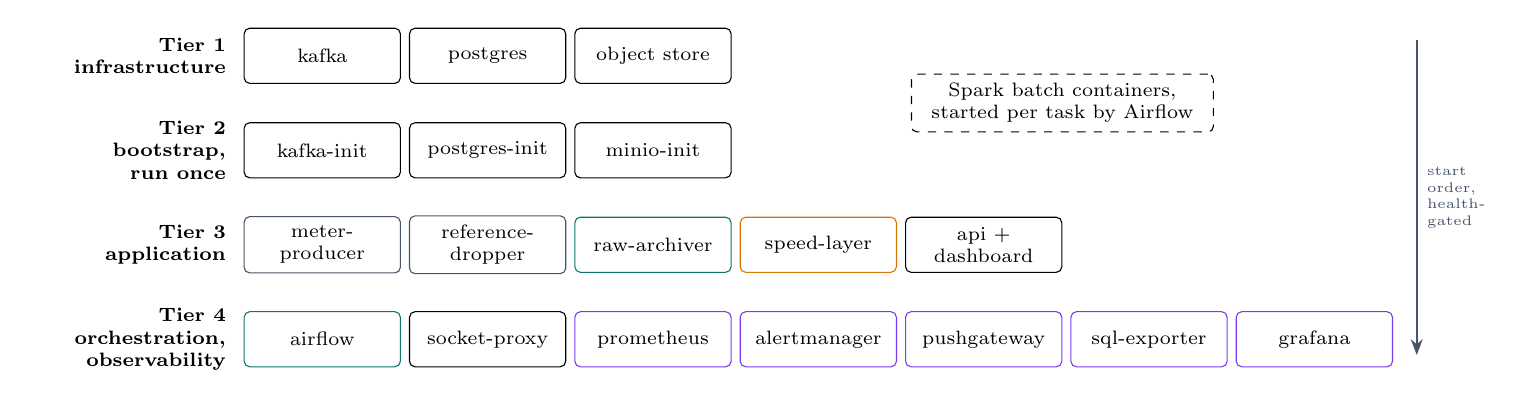
\begin{tikzpicture}[
  c/.style={draw, rounded corners=2pt, font=\scriptsize, align=center, minimum height=0.7cm,
            text width=1.75cm, fill=white}]
  \foreach \y/\t in {0/{Tier 1\\infrastructure}, -1.2/{Tier 2\\bootstrap, run once}, -2.4/{Tier 3\\application}, -3.6/{Tier 4\\orchestration, observability}}
    \node[font=\scriptsize\bfseries, align=right, anchor=east, text width=2.4cm] at (0.3,\y) {\t};
  \node[c] at (1.4,0) {kafka};
  \node[c] at (3.5,0) {postgres};
  \node[c] at (5.6,0) {object store};
  \node[c] at (1.4,-1.2) {kafka-init};
  \node[c] at (3.5,-1.2) {postgres-init};
  \node[c] at (5.6,-1.2) {minio-init};
  \node[c, draw=infrac] at (1.4,-2.4) {meter-producer};
  \node[c, draw=infrac] at (3.5,-2.4) {reference-dropper};
  \node[c, draw=batchc] at (5.6,-2.4) {raw-archiver};
  \node[c, draw=speedc] at (7.7,-2.4) {speed-layer};
  \node[c] at (9.8,-2.4) {api + dashboard};
  \node[c, draw=batchc] at (1.4,-3.6) {airflow};
  \node[c] at (3.5,-3.6) {socket-proxy};
  \node[c, draw=obsc] at (5.6,-3.6) {prometheus};
  \node[c, draw=obsc] at (7.7,-3.6) {alertmanager};
  \node[c, draw=obsc] at (9.8,-3.6) {pushgateway};
  \node[c, draw=obsc] at (11.9,-3.6) {sql-exporter};
  \node[c, draw=obsc] at (14.0,-3.6) {grafana};
  \node[c, dashed, text width=3.6cm] at (10.8,-0.6) {Spark batch containers,\\started per task by Airflow};
  \draw[-{Stealth[length=2mm]}, infrac, line width=0.8pt] (15.3,0.2) -- node[right, font=\tiny, align=left]{start\\order,\\health-\\gated} (15.3,-3.8);
\end{tikzpicture}}
\caption{Deployment topology: 18 containers in four health-gated tiers (15 long-running,
3 bootstrap). Billing, rollup and reconciliation run in short-lived Spark containers that
Airflow starts per task.}
\label{fig:deployment}
\end{figure}

Measured resource use on the demonstration laptop (sampled every 5\,s over 6.5 minutes
including a billing run): 5.3--6.1\,GiB of container memory at steady state and up to
6.4\,GiB during a billing run. The stack therefore needs about 9\,GB of memory allocated
to Docker to avoid swapping; the README states this as a prerequisite.

\subsection{Data Contracts}

The event contract was frozen before parallel implementation began, because three
components were built against it concurrently. Contracts are Pydantic models in
\texttt{voltstream/contracts/}, exported as JSON Schema and guarded by a drift test.

\begin{lstlisting}[caption={Event published to topic \texttt{meter.readings}, keyed by \texttt{household\_id}.},label={lst:event}]
{
  "schema_version": "1.0",     // forward-compatible evolution
  "event_id": "uuid4",         // idempotency safeguard
  "trace_id": "uuid4",         // also in Kafka headers; propagated end to end
  "meter_id": "MTR-0042",  "household_id": "HH-0042",  "grid_zone": "ZONE-C",
  "event_ts": "2026-01-02T14:15:00Z",   // SIMULATED time; drives all windowing
  "consumption_kwh": 0.412,  "solar_generation_kwh": 0.180,
  "voltage": 232.4,            // unused by billing; demonstrates column pruning
  "producer_id": "sim-01"
}
\end{lstlisting}

The daily tariff file (\texttt{tariff\_YYYY-MM-DD.csv}) supplies, per household,
\texttt{household\_id}, \texttt{billing\_tier}, \texttt{subsidy\_flag}, the three block
rates, the tier's fixed charge, the subsidy percentage, the export rate and an
\texttt{effective\_date}; the brief's single \texttt{tariff\_rate} is extended to block
rates so the billing logic is non-trivial. The weather file supplies \texttt{grid\_zone},
\texttt{forecast\_date}, \texttt{cloud\_cover\_pct} and \texttt{solar\_irradiance\_index}.
Both are dropped as CSV into the object-storage landing zone once per simulated day, and
every row is validated against its contract before use; an invalid row fails the run
naming its line.

\subsection{Serving Schema}

\begin{table}[H]
\centering
\caption{Serving-layer tables and their provenance.}
\label{tab:tables}
\small
\begin{tabularx}{\textwidth}{L{4.4cm} L{1.6cm} X}
\toprule
\textbf{Table} & \textbf{Written by} & \textbf{Purpose} \\
\midrule
\texttt{households} & Seed & The 50-household dimension: zone, tier, solar, subsidy \\
\texttt{zone\_metrics\_rt} & Speed & Per-zone windowed load and renewable ratio \\
\texttt{household\_running\_rt} & Speed & Provisional running total and estimated bill \\
\texttt{household\_bill\_daily} & Batch & Current authoritative bill with block breakdown \\
\texttt{household\_bill\_history} & Batch & Every billing run's bills, append-only (audit trail) \\
\texttt{zone\_metrics\_daily} & Batch & Exact daily zone rollup \\
\texttt{rejected\_records} & Both & Dead-lettered records with rejection reason and \texttt{trace\_id} \\
\texttt{pipeline\_runs} & Batch & Run ledger; the finalisation flag the merge reads \\
\texttt{reconciliation\_daily} & Batch & Speed-versus-batch divergence, split into tariff and data effects \\
\bottomrule
\end{tabularx}
\end{table}

The two views occupy \emph{separate tables}, so neither layer overwrites the other and
every row carries unambiguous provenance.

\subsection{Ingestion}

Two Python simulators provide the sources. The \textbf{meter producer} evaluates each
household's load and solar curves for the current simulated time (solar is zero from
18:00 to 06:00), adds stochastic noise, applies configured fault-injection rates and
publishes to Kafka on a fixed real-time tick grid so that exactly 150 readings per meter
per day are emitted even when a tick runs late. The \textbf{reference dropper} writes the
tariff and weather files for each simulated day as it closes; on start it also catches up
any closed days whose files are missing. Tariffs change day over day
(\texttt{block\_1\_rate} $\pm$ 0.50), so a stale tariff has a measurable effect on the
provisional bill.

\paragraph{Deliberate fault injection.} Robustness claims are unfalsifiable without
adverse data, so the producer emits---at independently configurable rates
(Table~\ref{tab:faultvals})---duplicate events, out-of-order events, nulls in required
fields, negative kWh values, unknown household identifiers and periodic meter dropouts
with store-and-forward backfill. Invalid records are routed to the dead-letter topic
\texttt{meter.readings.dlq} and recorded in \texttt{rejected\_records} with a categorised
reason, giving the alert rules genuine conditions to detect. Setting every rate to zero
yields output identical to input, which is asserted as a test.

\subsection{Processing}

\paragraph{Raw archiver.} Consumes from Kafka and writes Parquet to the master dataset
with \emph{no transformation whatsoever}, partitioned by simulated date and hour,
checkpointing its Kafka offsets on a named volume so it resumes where it stopped.

\paragraph{The guarantee is no loss, not exactly-once.} Kafka delivers at least once,
and a Spark file sink commits its data files and its offsets in two separate steps; a
kill between them leaves committed files whose offsets were never recorded, so the
restarted query re-reads that range. We measured this rather than assuming it
(Section~\ref{sec:res-resilience}): killing the archiver with \texttt{SIGKILL} mid-run
produced \textbf{334 duplicate rows out of 14{,}012}, with no lost \texttt{event\_id} and
no gap in the Kafka offsets on any partition. Duplicates are removed downstream by
deduplication on $(\mathit{meter\_id}, \mathit{event\_ts})$, which is why that key exists.
Claiming exactly-once here would be an overclaim the file sink does not support.

\paragraph{Speed layer.} Consumes the same topic independently of the archiver, validates
each record with \texttt{core/validation.py} (invalid ones to the DLQ), deduplicates on the
batch layer's key, assigns each reading to a 15-simulated-minute event-time tumbling window
under a \textbf{30-simulated-minute} watermark, aggregates by zone and by household, and
upserts into PostgreSQL through \texttt{foreachBatch} at a 10-real-second trigger in
\emph{update} output mode. Writes are bulk upserts per micro-batch rather than per-record
inserts. The provisional bill applies \texttt{core/spark\_expr.py} to the running totals
with yesterday's tariff.

\paragraph{Watermark units, and what actually governs lateness.} The watermark applies to
\texttt{event\_ts}, which advances at $288\times$ wall-clock, so it is expressed in
\emph{simulated} minutes: 30 simulated minutes is 6.25 real seconds. Stating it as ``30
seconds'' would be ambiguous in a way that changes behaviour. A more consequential
observation follows from the time compression: the 10-real-second trigger interval is 48
\emph{simulated} minutes---longer than the watermark. At this time scale the trigger
interval, not the watermark, dominates what gets dropped, and a watermark shorter than one
trigger is largely decorative. This is an artefact of compressing a day into five minutes
rather than a property of the architecture; Section~\ref{sec:res-recon} gives the
measurement. In update mode the watermark is also \emph{not} on the latency path: every
changed aggregate is emitted at the end of each micro-batch, and the watermark only decides
when state is evicted.

\paragraph{Batch layer.} The \texttt{daily\_billing} DAG runs eight tasks
(Figure~\ref{fig:timeline}): wait for the tariff; a 90-real-second late-data grace; the
Spark billing job, which reads the day's partition, validates, deduplicates on
$(\mathit{meter\_id}, \mathit{event\_ts})$, joins the day's tariff, applies the shared
netting and tariff functions and writes \texttt{household\_bill\_daily},
\texttt{household\_bill\_history} and a \texttt{success} row in \texttt{pipeline\_runs};
two verification tasks (row count equals the household count; every bill satisfies the
total identity); the exact daily zone rollup, with a cross-check that zone totals equal
household totals; reconciliation; and report generation.

\paragraph{Reconciliation.} For every household it decomposes the gap between the
speed estimate and the batch bill into a \emph{tariff effect} (the speed layer's kWh
re-priced at today's tariff, minus its estimate) and a \emph{data effect} (the batch bill
minus that re-priced figure---readings the speed layer never saw). By construction the
two sum exactly to the total divergence, which is asserted on every row.

\subsection{Runtime Behaviour}

\begin{figure}[H]
\centering
\resizebox{\textwidth}{!}{%
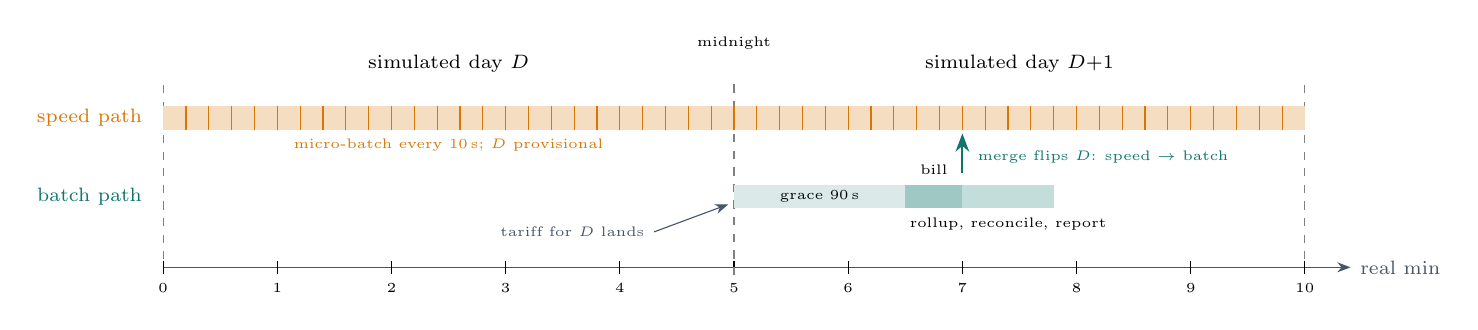
\begin{tikzpicture}[x=1.45cm]
  \draw[-{Stealth}, infrac] (0,0) -- (10.4,0) node[right, font=\scriptsize]{real min};
  \foreach \t in {0,...,10} \draw (\t,0.08) -- (\t,-0.08) node[below, font=\tiny]{\t};
  \node[font=\scriptsize, above] at (2.5,2.35) {simulated day $D$};
  \node[font=\scriptsize, above] at (7.5,2.35) {simulated day $D{+}1$};
  \draw[dashed, gray] (5,-0.1) -- (5,2.4) node[above, font=\tiny, black, yshift=7pt]{midnight};
  \draw[dashed, gray] (0,0.1) -- (0,2.4); \draw[dashed, gray] (10,0.1) -- (10,2.4);

  % speed path
  \node[font=\scriptsize, anchor=east, text=speedc] at (-0.1,1.9) {speed path};
  \fill[speedc!25] (0,1.75) rectangle (10,2.05);
  \foreach \t in {0.2,0.4,...,9.9} \draw[speedc] (\t,1.75) -- (\t,2.05);
  \node[font=\tiny, text=speedc] at (2.5,1.55) {micro-batch every 10\,s; $D$ provisional};

  % batch path for day D
  \node[font=\scriptsize, anchor=east, text=batchc] at (-0.1,0.9) {batch path};
  \fill[batchc!15] (5,0.75) rectangle (6.5,1.05); \node[font=\tiny] at (5.75,0.9) {grace 90\,s};
  \fill[batchc!40] (6.5,0.75) rectangle (7.0,1.05); \node[font=\tiny, above] at (6.75,1.05) {bill};
  \fill[batchc!25] (7.0,0.75) rectangle (7.8,1.05); \node[font=\tiny, below] at (7.4,0.75) {rollup, reconcile, report};
  \draw[-{Stealth}, infrac] (4.3,0.45) node[left, font=\tiny]{tariff for $D$ lands} -- (4.95,0.8);
  \draw[-{Stealth}, batchc, thick] (7.0,1.2) -- (7.0,1.7);
  \node[font=\tiny, text=batchc, align=left, anchor=west] at (7.05,1.4) {merge flips $D$: speed $\rightarrow$ batch};
\end{tikzpicture}}
\caption{One simulated day. The two paths run concurrently; neither waits for the other.
The batch timings shown are those measured in the Gate 4 run.}
\label{fig:timeline}
\end{figure}

\begin{table}[H]
\centering
\caption{Contrast between the two processing paths.}
\label{tab:paths}
\small
\begin{tabularx}{\textwidth}{L{2.8cm} X X}
\toprule
 & \textbf{Speed path} & \textbf{Batch path} \\
\midrule
Order & Process, then store & Store, then process \\
Reads from & Kafka (live) & Parquet (closed day) + day's tariff \\
Triggered by & Continuous micro-batches & Tariff file arrival (watcher DAG) \\
Latency (measured) & Mean 6.3\,s, p95 14.3\,s & $\sim$2.5 real min after day close \\
Late data & Discarded past watermark & Included; full rescan \\
Output & Approximate, provisional & Exact, authoritative \\
On failure & Dashboard gap; no data lost & Report delayed; rerun the DAG \\
\bottomrule
\end{tabularx}
\end{table}

\textbf{Neither path failing causes data loss}, because raw events persist in Kafka within
its retention window and in Parquet indefinitely. Failure produces delay, not loss---the
operational expression of why the master dataset exists. On restart, the stateless
components resume immediately; the two Spark jobs resume at their last committed offset
from checkpoints on named volumes; and Airflow does not repeat completed runs.

\subsection{Code Quality, Testing and Reproducibility}

The codebase is a typed Python 3.11 package (\texttt{src/voltstream/}) organised by layer:
\texttt{simulators/}, \texttt{streaming/}, \texttt{batch/}, \texttt{storage/},
\texttt{api/}, the shared \texttt{core/} and \texttt{contracts/}. All configuration lives in
\texttt{config/base.yaml}, validated at start-up by Pydantic, with environment-variable
overrides; no number reaching the billing arithmetic is hard-coded. The dashboard is plain
HTML, CSS and ES modules served by the API, with no build step.

The test suite contains \textbf{281 test functions} across unit, property-based
(Hypothesis), consistency and integration suites. Integration tests cover producer to
Kafka, the batch job end to end against committed fixtures with hand-computed bills, the
merge function, and archiver restart. The alert rules have their own \texttt{promtool}
unit tests, and a configuration test fails if the alert thresholds, metric names or
dashboard queries disagree with the code. GitHub Actions CI runs ruff, mypy, the tests
with the 100\% \texttt{core/} coverage gate, and the alert checks on every push.
The README gives prerequisites, a one-command start, a timeline of what to expect, every
demonstration scenario, and troubleshooting; \texttt{docs/runbook.md} is the demo script.

% =====================================================================
\section{Observability Design}
\label{sec:observability}
% =====================================================================

Observability answers three questions for an operator: \emph{is data flowing}, \emph{is it
correct}, and \emph{where is it stuck}. Each instrument below exists to answer one of them.

\begin{figure}[H]
\centering
\resizebox{0.95\textwidth}{!}{%
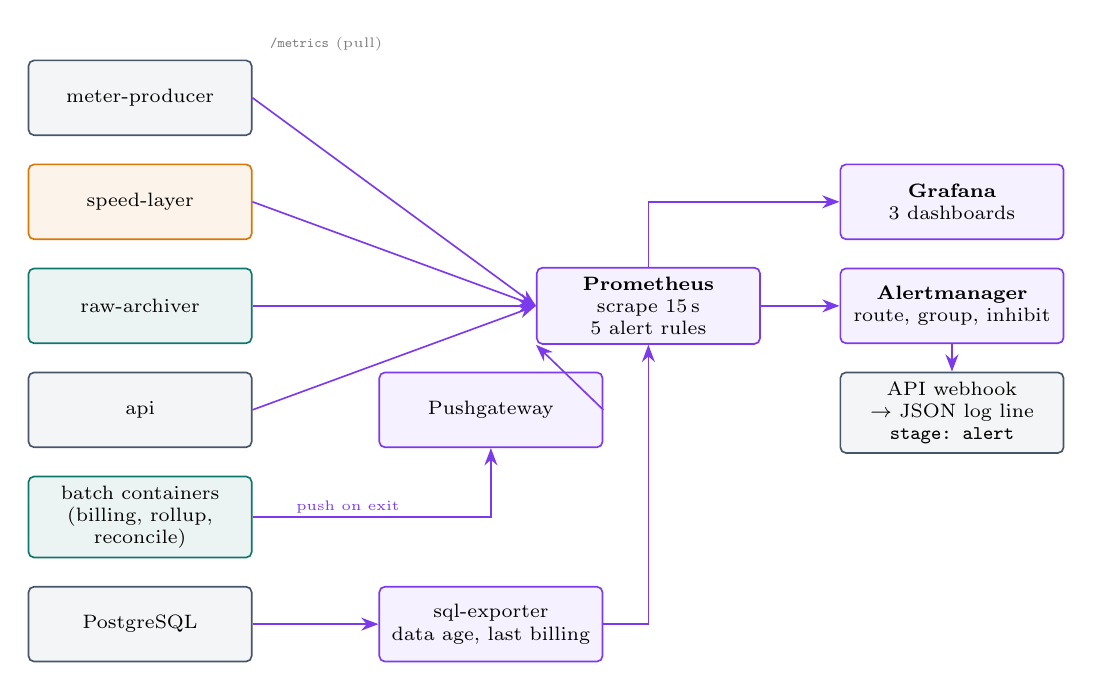
\begin{tikzpicture}[node distance=0.35cm and 1.0cm]
  \node[ibox] (prod) {meter-producer};
  \node[sbox, below=of prod] (speed) {speed-layer};
  \node[bbox, below=of speed] (arch) {raw-archiver};
  \node[ibox, below=of arch] (api) {api};
  \node[bbox, below=of api] (bat) {batch containers\\(billing, rollup, reconcile)};
  \node[ibox, below=of bat] (pg) {PostgreSQL};

  \node[obox, right=1.6cm of api] (pgw) {Pushgateway};
  \node[obox, right=1.6cm of pg] (sqle) {sql-exporter\\data age, last billing};
  \node[obox, right=3.6cm of arch] (prom) {\textbf{Prometheus}\\scrape 15\,s\\5 alert rules};
  \node[obox, right=of prom] (am) {\textbf{Alertmanager}\\route, group, inhibit};
  \node[obox, above=of am] (graf) {\textbf{Grafana}\\3 dashboards};
  \node[ibox, below=of am] (hook) {API webhook\\$\rightarrow$ JSON log line\\\texttt{stage: alert}};

  \foreach \n in {prod,speed,arch,api} \draw[arr, obsc] (\n.east) -- (prom.west);
  \draw[arr, obsc] (bat.east) -| node[lbl, pos=0.2, above]{push on exit} (pgw.south);
  \draw[arr, obsc] (pgw.east) -- (prom.south west);
  \draw[arr, obsc] (pg) -- (sqle);
  \draw[arr, obsc] (sqle.east) -| (prom.south);
  \draw[arr, obsc] (prom) -- (am);
  \draw[arr, obsc] (prom.north) |- (graf.west);
  \draw[arr, obsc] (am) -- (hook);
  \node[font=\tiny, text=gray, anchor=west] at ($(prod.north east)+(0.1,0.2)$) {\texttt{/metrics} (pull)};
\end{tikzpicture}}
\caption{Observability instrumentation. Long-running services are scraped; batch
containers push; two facts only the database knows are exported by \texttt{sql-exporter};
alerts return to the API as structured log lines and to the dashboard's alert banner.
Grafana also reads PostgreSQL through a read-only role. Every service writes JSON logs to stdout.}
\label{fig:observability}
\end{figure}

\subsection{Structured Logging}

Every service emits one JSON object per line to stdout through \texttt{logging\_setup.py},
under a fixed envelope:

\begin{lstlisting}[caption={A speed-layer log line.},label={lst:log}]
{"ts": "2026-09-27T13:35:25.992Z", "level": "INFO", "service": "speed-layer",
 "stage": "speed-zone", "trace_id": "...", "sim_date": "2026-01-01",
 "msg": "zone windows upserted", "batch_id": 42, "rows_out": 15}
\end{lstlisting}

\texttt{ts} is real time; \texttt{sim\_date} is the simulated day. \texttt{service} and
\texttt{stage} identify where in the pipeline a line came from---ingestion
(\texttt{producer}), processing (\texttt{speed-zone}, \texttt{archive}, \texttt{billing},
\dots) and storage/serving (\texttt{api}). Structured rather than free-text logging is used
because it is machine-parseable, filterable by correlation identifier with one
\texttt{jq} expression, and survives later shipment to an aggregator without reformatting.
\textbf{Alerts are log lines too}: Alertmanager's receiver is the API's webhook, which
logs every notification with \texttt{stage: alert}, so the API log doubles as the pager.

\subsection{Metrics}

\begin{table}[H]
\centering
\caption{Exported metrics and the question each answers. All eight application metrics are
defined in one module, \texttt{metrics.py}; the last two rows come from
\texttt{sql-exporter}.}
\label{tab:metrics}
\small
\begin{tabularx}{\textwidth}{L{5.6cm} L{1.5cm} L{2.2cm} X}
\toprule
\textbf{Metric} (prefix \texttt{voltstream\_}) & \textbf{Type} & \textbf{Labels} & \textbf{Answers} \\
\midrule
\texttt{events\_produced\_total} & Counter & producer & Is the source alive? \\
\texttt{events\_consumed\_total} & Counter & layer & Is each consumer keeping pace? \\
\texttt{records\_rejected\_total} & Counter & layer, reason & What kind of bad data, how much? \\
\texttt{e2e\_latency\_seconds} & Histogram & layer & Where does latency accumulate? \\
\texttt{consumer\_lag} & Gauge & layer, partition & Is a branch falling behind? \\
\texttt{zone\_renewable\_ratio} & Gauge & zone & Business metric; drives an alert \\
\texttt{batch\_duration\_seconds} & Histogram & job & Is the nightly job degrading? \\
\texttt{lambda\_divergence} & Gauge & --- & Are the two layers agreeing? \\
\addlinespace
\texttt{pg\_zone\_data\_age\_seconds} & Gauge & zone & Has a zone stopped reporting? \\
\texttt{pg\_billing\_last\_success\_timestamp\_seconds} & Gauge & --- & When was a day last billed? \\
\bottomrule
\end{tabularx}
\end{table}

Three deserve comment. \texttt{e2e\_latency\_seconds} runs from the Kafka record timestamp
to the sink commit (the zone view committed to PostgreSQL, which is what the dashboard
reads), so the latency budget is \emph{measured} rather than asserted
(Section~\ref{sec:res-latency}). \texttt{lambda\_divergence} is the mean percentage gap
between speed estimate and batch final, pushed by reconciliation, so the system monitors
its own architectural weakness. The two database-derived gauges exist because two alerts
need facts no application metric carries: the renewable ratio sits at a constant 0 all
night, so an unchanged value cannot distinguish a dead feed from darkness, and only the
run ledger knows when billing last succeeded (decision D9).

\subsection{Tracing}
\label{sec:tracing}

True distributed tracing through Spark executors, with spans crossing the JVM and Python
boundary inside a micro-batch, is impractical within this project's scope. We implement
\textbf{correlation-identifier tracing} instead: a \texttt{trace\_id} is generated at the
producer, carried in Kafka message headers, propagated into the master dataset and the
dead-letter topic, and emitted in every log line at every stage, alongside the end-to-end
latency histogram. The API extends the idea to requests: it accepts a caller's
\texttt{X-Trace-Id} or mints one, binds it to every log line of the request and echoes it
in the response. Any record's path and timing across the pipeline can be reconstructed by
filtering on one identifier. This is a deliberate trade: a partially functional
distributed-tracing deployment would demonstrate less than a complete correlation-based
implementation whose limitation is stated.

\subsection{Alert Rules}
\label{sec:alerts}

Alert rules are declarative files in the repository (\texttt{config/prometheus/}), with
thresholds mirrored from the \texttt{alerts:} block of \texttt{base.yaml} and a test that
fails if the two disagree. Time in the rules is real time.

\begin{table}[H]
\centering
\caption{Alert rules and the failure each detects.}
\label{tab:alerts}
\small
\begin{tabularx}{\textwidth}{L{3.9cm} L{1.4cm} X}
\toprule
\textbf{Rule} & \textbf{Severity} & \textbf{Condition and purpose} \\
\midrule
\texttt{MeterDataStale} & critical & A zone's newest window older than 2 real minutes (for 30\,s); producer or speed-layer failure \\
\texttt{LowRenewableContribution} & warning & Zone renewable ratio below 15\% for three consecutive windows; the business alert required by the brief \\
\texttt{HighRejectRate} & warning & Speed-layer rejects exceed 5\% of consumed records over 5 minutes (for 1\,m); upstream data-quality regression \\
\texttt{BatchSLAMiss} & critical & No successful billing run within 10 real minutes of a day's close; orchestration failure \\
\texttt{LambdaDivergenceHigh} & warning & Mean speed-versus-batch divergence above 5\% on the latest reconciled day; logic drift or excessive data loss between layers \\
\bottomrule
\end{tabularx}
\end{table}

\begin{lstlisting}[caption={The business alert as deployed (\texttt{alert\_rules.yml}).},label={lst:alert}]
- alert: LowRenewableContribution
  expr: voltstream_zone_renewable_ratio < 0.15
  for: 10s          # 3 windows = 45 sim min = 9.4 real s
  labels:      { severity: warning }
  annotations: { summary: "{{ $labels.grid_zone }} renewable ratio {{ $value | humanizePercentage }}, below 15%" }
\end{lstlisting}

Alertmanager routes \texttt{critical} and \texttt{warning} separately and applies one
\textbf{inhibition}: \texttt{MeterDataStale} for a zone suppresses that zone's
\texttt{LowRenewableContribution}, because no data explains no solar. The API also exposes
\texttt{/health/live}, \texttt{/health/ready} (PostgreSQL and object storage reachable;
Alertmanager deliberately excluded, so a monitoring outage never becomes a serving
outage) and \texttt{/api/v1/alerts/status}, which surfaces firing alerts to the dashboard
and reports ``unknown'' rather than ``none'' when Alertmanager is unreachable.

Three Grafana dashboards are provisioned: \emph{pipeline health} (throughput per stage,
consumer lag, rejects by reason, latency quantiles, alerts firing), \emph{grid operations}
(load, solar and renewable ratio by zone) and \emph{Lambda divergence} (estimate versus
final over time, split into tariff and data effects).

% =====================================================================
\section{Results}
\label{sec:results}
% =====================================================================

All results below come from runs of the complete Compose stack on one Windows laptop
(Docker Desktop, 16 CPUs, $\sim$7.5\,GiB for Docker). The reference run is \emph{Gate 4}
(27 September 2026), the first uninterrupted run with both Lambda paths live; drills were
run on 28 September. Figures are quoted from the recorded evidence in
\texttt{docs/assumptions.md}, \texttt{docs/runbook.md} and
\texttt{docs/architecture/04-observability.md}. The verification script
\texttt{voltstream.ps1 check -Date 2026-01-02} reported \textbf{37 passed, 0 failed} on the
reference run.

\subsection{Real-Time Zone Monitoring}
\label{sec:res-live}

In 40 real seconds the newest zone window advanced from 07:30 to 10:45 simulated (3\,h
15\,min, i.e.\ $288\times$) and \texttt{zone\_metrics\_rt} grew from 119 to 180 rows. The
Live grid tab (Figure~\ref{fig:live}) polls \texttt{/api/v1/zones/load} every 5 seconds
and shows grid load, solar generation, renewable share and active meters per zone. Renewable
share falls to 0\% every simulated night and recovers after dawn (the Grafana grid-operations dashboard plots the same series against the 15\% threshold), which is exactly the
condition \texttt{LowRenewableContribution} reports.

\begin{lstlisting}[caption={\texttt{GET /api/v1/zones/load}: shape of one zone's entry (\texttt{api/models.py}).},label={lst:zone}]
{"grid_zone": str, "window_start": datetime, "window_end": datetime,        // simulated time
 "total_consumption_kwh": Decimal, "total_solar_kwh": Decimal,
 "renewable_ratio": Decimal,  "active_meters": int}                          // one per zone
\end{lstlisting}

\begin{figure}[H]
\centering
\shot{dashboard}{Dashboard, Live grid tab: KPI tiles, grid load vs solar, zones compared,
zone cards}{5.8cm}
\caption{Live grid (speed layer): the real-time answer to ``grid load and renewable
contribution by zone''.}
\label{fig:live}
\end{figure}

\subsection{Daily Per-Household Billing and Solar Report}
\label{sec:res-report}

For 2026-01-02, the first complete day, the batch layer read \textbf{7{,}029 rows} from
the master dataset and wrote \textbf{50 bills}; \texttt{pipeline\_runs} records the run as
\texttt{success}, and the whole eight-task DAG took \textbf{59\,s}. Every bill satisfies
$\mathit{total} = \mathit{energy} + \mathit{fixed} - \mathit{subsidy} - \mathit{export}$.
The day's consolidated report (\texttt{voltstream-archive/reports/report\_2026-01-02.md},
status FINAL) is generated by the last DAG task and contains, in order: grid operations by
zone (consumption, solar, self-consumed, exported, renewable share, peak, meters), billing
totals (households billed, kWh, total billed, readings processed, duplicates removed), data
quality (rejected records by reason), speed versus batch (mean divergence), and the pipeline
run ledger. The same content is served by \texttt{/api/v1/reports/daily} (every endpoint is listed in the generated OpenAPI reference at \texttt{/docs}) and rendered by
the dashboard's Daily report tab (Figure~\ref{fig:report}). Per household, the Household
bills tab shows the waterfall from energy charge to total, the energy flow (own solar used,
grid import, export), the block-by-block tariff and the bill's lineage
(Figure~\ref{fig:bills}).

\begin{figure}[H]
\centering
\shot{dashboard-report}{Dashboard, Daily report tab for 2026-01-02: tiles, zone totals,
rejected records, billing runs (take by hand: \#/report)}{5.8cm}
\caption{The consolidated daily report for one simulated day.}
\label{fig:report}
\end{figure}

\subsection{Provisional-to-Final Transition}
\label{sec:res-merge}

The same request, \texttt{GET /api/v1/households/HH-0001/bill?date=2026-01-02}, was issued
before and after the day was billed:

\begin{table}[H]
\centering
\caption{The merge function flipping for one household and date (Gate 4 run).}
\label{tab:flip}
\small
\begin{tabularx}{\textwidth}{L{3.2cm} X X X}
\toprule
 & \textbf{Mid-day (12:54:13)} & \textbf{At day close} & \textbf{After billing (12:57:33)} \\
\midrule
\texttt{source} & \texttt{speed} & \texttt{speed} & \texttt{batch} \\
\texttt{provisional} & \texttt{true} & \texttt{true} & \texttt{false} \\
Tariff used & 2026-01-01 & 2026-01-01 & 2026-01-02 \\
Energy & 10.0665 kWh so far & --- & 13.4363 kWh, 138 readings, 3 duplicates removed \\
Total & 200.53 & 227.49 & \textbf{234.21} \\
\bottomrule
\end{tabularx}
\end{table}

The final bill exceeded the day-close estimate by 6.72, which is \textbf{2.869\%} of the
gross charges; reconciliation attributes it almost entirely to the stale tariff, since
2026-01-02's tariff was dearer than the one the speed layer used. A repeat on 28 September
(\texttt{voltstream.ps1 demo}, 6\textonequarter{} minutes end to end) gave the same shape:
final 237.38, delta $-6.90$, all of it tariff effect, 2.907\%. The dashboard badge flips from
\emph{Provisional (speed)} to \emph{Final (batch)} in place while the page is open
(Figure~\ref{fig:bills}).

\begin{figure}[H]
\centering
\begin{subfigure}{0.49\textwidth}
  \centering
  \shot{dashboard-bills-provisional}{Household bills, day open: badge
  Provisional (speed)}{5cm}
  \caption{Before finalisation.}
\end{subfigure}\hfill
\begin{subfigure}{0.49\textwidth}
  \centering
  \shot{dashboard-bills-final}{Household bills, same household and date: badge Final
  (batch), estimate vs final}{5cm}
  \caption{After finalisation.}
\end{subfigure}
\caption{The merge function as the user sees it.}
\label{fig:bills}
\end{figure}

\subsection{Speed-versus-Batch Reconciliation}
\label{sec:res-recon}

\begin{table}[H]
\centering
\caption{Measured attribution of the divergence (Gate 4 run, 50 households per day).
Day 1 is partial because the stack starts at simulated midnight; quote day 2.}
\label{tab:recon}
\small
\begin{tabularx}{\textwidth}{L{2.1cm} X X X X X X}
\toprule
\textbf{Day} & \textbf{Mean tariff effect} & \textbf{Mean data effect} & \textbf{Tariff share} &
\textbf{Mean div.} & \textbf{Max div.} & \textbf{Speed kWh shortfall} \\
\midrule
2026-01-01 & $+5.14$ & $-0.89$ & 85.2\% & 1.570\% & 3.537\% & 0.861\% \\
2026-01-02 & $-5.35$ & $-0.61$ & 89.7\% & 1.878\% & 4.450\% & 0.523\% \\
\bottomrule
\end{tabularx}
\end{table}

The tariff effect is non-zero for all 50 households and alternates in sign day by day, as
the tariff generator alternates \texttt{block\_1\_rate} up and down. The data effect is
non-zero for 10--12 households per day, all negative: readings flushed by meter dropouts
arrive later than the watermark, so the speed layer drops them and the batch layer bills
them. The daily energy gap of \textbf{0.52\%} sits inside the design's 0.25--5\% acceptance
band. Mean divergence (1.88\%) stays well under the 5\% \texttt{LambdaDivergenceHigh}
threshold in normal running (Figure~\ref{fig:divergence}).

At the 15-minute grain the operational view was short by \textbf{1.16\%} of the day's
energy with the default fault configuration, and by 1.00\% with dropouts disabled---so most
of the 15-minute gap comes from ordinary reordering, not from dropout backfill. The design
had predicted the opposite, reasoning that reordering bounded by the 30-minute watermark
would always be absorbed. The measurement refuted that prediction; the cause is the
48-simulated-minute trigger discussed in Section~\ref{sec:implementation}.

\begin{figure}[H]
\centering
\shot{grafana-lambda-divergence}{Grafana, Lambda divergence dashboard: mean divergence per
reconciled day, tariff vs data effect}{5.8cm}
\caption{Speed-versus-batch divergence tracked over time.}
\label{fig:divergence}
\end{figure}

\subsection{Observability in Operation}
\label{sec:res-alerts}

Each alert was triggered by a scripted fault (\texttt{voltstream.ps1 faults}), asserted
through Alertmanager's API, and the fault undone:

\begin{table}[H]
\centering
\caption{Measured firing behaviour of every alert rule under an induced fault.}
\label{tab:firing}
\small
\begin{tabularx}{\textwidth}{L{3.4cm} L{3.4cm} X}
\toprule
\textbf{Rule} & \textbf{Induced fault} & \textbf{Measured} \\
\midrule
\texttt{MeterDataStale} & Producer stopped & Fired 173\,s and 195\,s after the stop, all 5 zones in one critical notification; resolved 41--46\,s after restart. At night, the zones' \texttt{LowRenewableContribution} alerts were inhibited as designed \\
\texttt{HighRejectRate} & 15\% null fields (normally 1\%) & Fired 119\,s after the change at a 5-minute reject ratio of 11.6\% (normal: $\sim$2\%) \\
\texttt{BatchSLAMiss} & \texttt{daily\_billing} paused & Fired 21\,s after its due time; resolved 6\,s after the first successful run once unpaused, the DAG catching up in $\sim$3 minutes \\
\texttt{LowRenewableContribution} & None: simulated night & Fired at simulated 19:40 (dusk) for all 5 zones; cleared at simulated 10:00 \\
\texttt{LambdaDivergenceHigh} & 60\% of readings 3--5 simulated hours late & \emph{Not reached live}: the reconciliation run stalled on memory on the demo laptop. Shown instead by lowering the threshold to 1\%: fired at the next evaluation on the observed 1.68\% and reached the webhook on the warning route \\
\bottomrule
\end{tabularx}
\end{table}

\begin{figure}[H]
\centering
\shot{stale-grafana-pipeline-health}{Grafana, pipeline health during the stale-data drill:
throughput drop, lag, alerts firing (faults -Capture)}{5.8cm}
\caption{Pipeline-health dashboard while \texttt{MeterDataStale} fires.}
\label{fig:health}
\end{figure}

\begin{figure}[H]
\centering
\begin{subfigure}{0.49\textwidth}
  \centering
  \shot{stale-alertmanager}{Alertmanager: MeterDataStale, all five zones}{4.5cm}
  \caption{Alertmanager.}
\end{subfigure}\hfill
\begin{subfigure}{0.49\textwidth}
  \centering
  \shot{rejects-prometheus-alerts}{Prometheus alerts page: HighRejectRate firing}{4.5cm}
  \caption{Prometheus rule state.}
\end{subfigure}
\caption{Alerts reaching the alerting stack under induced faults.}
\label{fig:alerts}
\end{figure}

A rejected record keeps its identity across stages: in Gate 3, 53 rows in
\texttt{rejected\_records} matched 53 messages in the DLQ exactly (27 \texttt{null\_field},
13 \texttt{negative\_kwh}, 13 \texttt{unknown\_household}), and a single \texttt{trace\_id}
was found in both the PostgreSQL row and the DLQ message.

\subsection{Resilience: Crashing Each Path}
\label{sec:res-resilience}

\paragraph{Raw archiver.} \texttt{SIGKILL}, 20\,s outage, restart: 10{,}661 rows before the
kill, 14{,}012 after recovery, 13{,}678 distinct \texttt{event\_id}s, 334 duplicates,
contiguous offsets on 3 of 3 partitions. No loss; duplicates as predicted by at-least-once
delivery and removed by the batch deduplication.

\paragraph{Speed layer.} During a 60\,s \texttt{SIGKILL} outage the live view went 56\,s
stale while the raw archiver took in 1{,}526 readings. The speed layer resumed from its
checkpoint and caught up 22\,s after restarting. The finalised bill for the previous day
stayed 237.38 before, during and after, and the day of the kill was billed in full (50 bills;
HH-0001 with 148 readings). Losing the fast layer cost freshness, never correctness.

\subsection{Restatement Demonstration}
\label{sec:res-restate}

\texttt{voltstream.ps1 backfill -Date 2026-01-02} corrupted that day's tariff file
(\texttt{block\_1\_rate} $+45.00$), restated the day, restored the file and restated
again. The corrupted run made all 50 bills wrong---the day's total went from
\textbf{18{,}737.41} to \textbf{44{,}876.57}---and the corrected run returned all 50 to the
cent. The ledger ended \texttt{superseded} $\rightarrow$ \texttt{superseded} $\rightarrow$
\texttt{success}, each row naming its own Airflow run (\texttt{billing\_\_2026-01-02},
\texttt{\dots\_\_r1}, \texttt{\dots\_\_r2}), and \texttt{household\_bill\_history} keeps all
three versions of every bill. The batch layer never patched a bill; it recomputed the day
from the immutable master dataset. (One corrected attempt failed on the memory-starved host
and Airflow's retry succeeded---the script reports such retries rather than hiding them.)

\begin{figure}[H]
\centering
\shot{airflow-daily-billing}{Airflow, daily\_billing graph: the eight tasks green (take by
hand; Airflow needs a login)}{5cm}
\caption{The \texttt{daily\_billing} DAG.}
\label{fig:airflow}
\end{figure}

\subsection{Measured Latency Budget}
\label{sec:res-latency}

\begin{table}[H]
\centering
\caption{End-to-end latency from \texttt{voltstream\_e2e\_latency\_seconds}, 20 minutes of
normal running (including four billing runs and a producer outage). API reads timed with 40
requests each.}
\label{tab:latency}
\small
\begin{tabularx}{\textwidth}{L{4.6cm} L{3.6cm} X}
\toprule
\textbf{Stage} & \textbf{Design estimate} & \textbf{Measured} \\
\midrule
Kafka $\rightarrow$ zone view committed (speed) & $\sim$40\,s & mean \textbf{6.3\,s}; p50 5.1\,s; p95 14.3\,s; p99 $\approx$45\,s; 0 of $\sim$2{,}300 over 60\,s \\
Kafka $\rightarrow$ Parquet committed (archiver) & --- & mean 3.0\,s; p50 1.0\,s; p95 13.3\,s; 0.15\% over 60\,s \\
Micro-batch trigger wait & $\sim$10\,s & 0--10\,s, 5\,s on average: the dominant term \\
Watermark wait & $\sim$30\,s & \textbf{0\,s} in update mode (the estimate was wrong) \\
API read, \texttt{/zones/load} & 20--50\,ms & p50 14.7\,ms; p95 32.2\,ms \\
API read, \texttt{/households/\{id\}/bill} & 20--50\,ms & p50 8.7\,ms; p95 13.3\,ms \\
\bottomrule
\end{tabularx}
\end{table}

The speed path met the 60\,s requirement on every observation, typically in about 5\,s. The
p99 tail came from a handful of micro-batches that coincided with billing runs, when the
batch Spark containers and the streaming drivers competed for the same laptop's CPU.

% =====================================================================
\section{Discussion}
\label{sec:discussion}
% =====================================================================

\subsection{Validity of the Architecture Decision}

The implementation bore out the decision's central argument. The provisional bill was
\emph{necessarily} wrong---it had to use yesterday's tariff---and the batch layer corrected
it within about 2.5 real minutes of the day closing, which a single streaming path could
only have matched by waiting for the tariff and thereby giving up the live estimate. The
restatement drill exercised exactly the capability that decided against Kappa: a day was
recomputed from Parquet after the fact, with the corrupt and corrected versions retained,
independently of Kafka's retention. The cost Lambda was expected to impose also
materialised: two processing jobs, an orchestrator and a reconciliation stage. The shared
\texttt{core/} module kept that cost to input divergence only---in every reconciled row the
tariff and data effects sum exactly to the total, and no divergence came from logic.

\subsection{Observed Latency Distribution}

The design predicted latency would accumulate in the watermark ($\sim$30\,s). It does not:
in update output mode the watermark governs state eviction, not emission, and the dominant
term is the 10\,s trigger interval. Measured median latency (5.1\,s) is almost exactly half
a trigger. The one design estimate that was clearly wrong was therefore also the one that
mattered least, since the corrected picture is an order of magnitude better than the
requirement. Tail latency is a resource-contention effect of running both layers on one
machine, not of the pipeline design.

\subsection{Speed-versus-Batch Divergence}

Divergence averaged 1.6--1.9\% of gross charges, about 85--90\% of it the stale tariff. That
is the intended behaviour: the speed layer is paid to be early, not exact. The remaining data
effect is the readings the speed layer drops. The finding we did not expect is that
reordering \emph{within} the watermark is dropped at the 15-minute grain, because at
$288\times$ compression one trigger spans 48 simulated minutes while the watermark is 30.
We have recorded rather than tuned this: raising the watermark above one trigger (60
simulated minutes) is the fix, but the measured result demonstrates the limits of time
compression more usefully than a tuned number would.

\subsection{What Observability Caught, and What It Would Miss}

Every induced fault was detected by the rule designed for it, with the stated severity and
with inhibition preventing a misleading second alert. Two gaps remain. \texttt{sql-exporter}
is a single point of silence: if it or PostgreSQL stops, \texttt{MeterDataStale} and
\texttt{BatchSLAMiss} go quiet rather than firing (the target shows as down on the
pipeline-health dashboard, but there is no dedicated alert). And the Pushgateway holds the
last divergence value indefinitely, so a reconciliation job that stops running would leave a
stale but healthy-looking gauge.

% =====================================================================
\section{Limitations and Production-Scale Considerations}
\label{sec:limitations}
% =====================================================================

The following simplifications were conscious decisions rather than oversights; the full
list, with measurements, is in \texttt{docs/assumptions.md}.

\subsection{Simulation Fidelity}

\begin{itemize}
  \item \textbf{Time compression scales event time but not processing time.} Network
        latency, garbage-collection pauses and micro-batch intervals proceed at
        wall-clock speed, so watermark tuning is not representative of production,
        where watermarks derive from empirically observed lateness distributions. The
        trigger-versus-watermark finding above is a direct consequence.
  \item \textbf{Interval readings rather than cumulative registers.} Real meters report
        a cumulative register; production would require per-meter stateful
        differencing with meter-reset and rollover detection.
  \item \textbf{Deterministic curves with additive noise} rather than measured data.
        The daily weather file is produced and landed but, as built, nothing consumes it:
        solar output does not depend on forecast cloud cover, and no bill depends on the
        weather.
  \item \textbf{Scale.} Fifty households across five zones is three to four orders of
        magnitude below a real utility deployment. Tariff values are synthetic.
\end{itemize}

\subsection{Architecture, Storage and Operations}

\begin{itemize}
  \item \textbf{Small-file problem.} Measured over one complete simulated day:
        \textbf{245 Parquet files averaging 10.2\,kB} across 24 hour partitions, against a
        row-group target of roughly 128\,MB. A streaming sink commits at least one file per
        partition per micro-batch. Production requires compaction, or a table format that
        compacts as part of its commit protocol.
  \item \textbf{Object-store commit protocol.} The default committer relies on rename,
        which object stores implement as copy-then-delete; production requires the S3A
        magic committer or a table format.
  \item \textbf{No schema registry.} Schema agreement is by convention, enforced by
        validation at the ingestion boundary and a JSON-Schema drift test.
  \item \textbf{Simplified dimension handling.} The tariff dimension uses an
        effective-dated join rather than a full slowly-changing-dimension implementation.
  \item \textbf{Single points of failure.} Single-broker Kafka, single-node Spark and a
        single PostgreSQL instance, with no replication or failover. Secrets are local
        defaults in \texttt{.env}.
  \item \textbf{Resource ceiling.} The whole stack needs about 9\,GB; with less, the batch
        Spark container can stall and be retried, which is why the divergence drill could
        not be shown live.
  \item \textbf{Driver-side Spark metrics and correlation-ID tracing}
        (Section~\ref{sec:tracing}); counts are exact, per-executor attribution is not
        available.
  \item \textbf{Object store dependency.} The MinIO-compatible fork is maintained by a
        single person; because only the S3 API is used, swapping it (e.g.\ for SeaweedFS or
        AWS S3) is configuration.
\end{itemize}

\subsection{Scale Boundary of the Serving Layer}

PostgreSQL is appropriate at our data volume and would remain so up to roughly the low
millions of aggregate rows per day. Beyond that the serving layer should migrate to a
time-series or columnar analytical store such as TimescaleDB or ClickHouse. Selecting
PostgreSQL reflects our actual data volume rather than aspirational scale.

\subsection{What We Would Change at Production Scale}

\begin{table}[H]
\centering
\caption{Production-scale evolution of the current design.}
\label{tab:production}
\small
\begin{tabularx}{\textwidth}{L{4.0cm} X}
\toprule
\textbf{Change} & \textbf{Motivation} \\
\midrule
Iceberg or Delta Lake over raw Parquet & ACID commits, time travel, schema evolution and
automatic compaction; removes the small-file and commit problems \\
Schema registry with Avro or Protobuf & Enforces backward-compatible evolution;
producer--consumer drift is a common production failure \\
Change data capture replacing file drops & Streaming tariff changes directly from the
billing system removes the daily-file dependency \\
Replicated Kafka, Spark on Kubernetes & Removes single points of failure; batch capacity
appears at day close and disappears afterwards, off the streaming nodes \\
Watermark set from measured lateness & At real time scale, with the trigger far shorter
than the watermark, reordering is absorbed as designed \\
Alert on exporter and Pushgateway staleness & Closes the two silent-failure gaps found in
Section~\ref{sec:discussion} \\
\bottomrule
\end{tabularx}
\end{table}

\paragraph{The architectural consequence.} Iceberg and Kafka tiered storage both remove the
retention constraint identified in Section~\ref{sec:arch} as the decisive argument for
Lambda. Once the log itself is durable, queryable and unbounded, Kappa's single codebase
becomes the better trade and we would migrate. The decision is correct \emph{given the
constraints as they stand}, and we can name precisely the change that would reverse it.

\paragraph{Functional extensions.} Joining the already-landed weather forecast to each
zone's historical solar profile would permit predicting renewable shortfall an hour
ahead---turning monitoring into decision support in which the operator pre-ramps generation
rather than reacting. Theft detection through deviation from a household's own baseline, and
demand-response simulation, are natural further extensions.

% =====================================================================
\section{Conclusion}
\label{sec:conclusion}
% =====================================================================

A utility needs the same smart-meter stream to answer two questions with opposite needs:
grid load and renewable share by zone within seconds, and an exact, auditable bill that
cannot exist until the day's tariff arrives. We chose a Lambda architecture because billing
must be restatable long after Kafka's retention has expired, which requires a master dataset
independent of the message bus, and we contained Lambda's principal risk by sharing all
billing logic between the layers through one pure module pinned by a consistency test.

Voltstream implements that design end to end with Kafka, Spark Structured Streaming and
batch, Parquet on object storage, PostgreSQL, Airflow and FastAPI, reproducible with one
command. On the running system the speed path delivered zone metrics in about 6\,s against a
60\,s budget; the batch layer finalised all 50 bills about 2.5 minutes after each simulated
day closed; the merge function flipped from provisional to final in front of the user; a
corrupted day was restated from the master dataset with its history retained; neither path's
crash lost data; and all five alert rules fired under the faults designed to trigger them.

The most significant limitation is that time compression distorts streaming behaviour: at
$288\times$ the trigger interval outgrows the watermark, and the speed view drops about 1\%
of each day's energy that a real-time-scale deployment would keep. The decision itself is
contingent: should the log become durable and queryable without bound, through tiered
storage or a table format, Kappa would become the better trade.

\clearpage
\phantomsection
\addcontentsline{toc}{section}{References}
\begin{thebibliography}{9}

\bibitem{marz}
N. Marz and J. Warren, \emph{Big Data: Principles and Best Practices of Scalable
Real-Time Data Systems}. Shelter Island, NY: Manning Publications, 2015.

\bibitem{kreps}
J. Kreps, ``Questioning the Lambda Architecture,'' O'Reilly Radar, 2014.

\bibitem{kafka}
Apache Software Foundation, \emph{Apache Kafka Documentation}. [Online]. Available:
\url{https://kafka.apache.org/documentation/}

\bibitem{spark}
Apache Software Foundation, \emph{Structured Streaming Programming Guide}. [Online].
Available: \url{https://spark.apache.org/docs/latest/structured-streaming-programming-guide.html}

\bibitem{airflow}
Apache Software Foundation, \emph{Apache Airflow Documentation}. [Online]. Available:
\url{https://airflow.apache.org/docs/}

\bibitem{parquet}
Apache Software Foundation, \emph{Apache Parquet Documentation}. [Online]. Available:
\url{https://parquet.apache.org/docs/}

\bibitem{prometheus}
Prometheus Authors, \emph{Prometheus Documentation}. [Online]. Available:
\url{https://prometheus.io/docs/}

\end{thebibliography}

% =====================================================================
\clearpage
\phantomsection
\addcontentsline{toc}{section}{Appendix A: Assumptions and Simplifications}
\section*{Appendix A: Assumptions and Simplifications}

\begin{enumerate}[itemsep=2pt]
  \item Simulated time is compressed by a factor of 288, so one simulated day elapses
        in five real minutes, starting at 2026-01-01 00:00 UTC when the stack starts
        (Section~\ref{sec:simclock}).
  \item Meters emit interval energy in kWh rather than cumulative register readings.
  \item Tariff block boundaries, rates, fixed charges and the subsidy percentage are
        synthetic values chosen to exercise the tiered billing logic
        (Table~\ref{tab:tariffvals}); they are not drawn from a published tariff
        schedule. Only the \emph{boundaries} are configuration; every rate reaches the
        billing logic through the day's tariff file.
  \item Fifty households are distributed across five grid zones with fixed membership.
  \item Fault-injection rates (Table~\ref{tab:faultvals}) exercise validation and
        alerting paths and do not represent realistic meter failure rates.
  \item Kafka retention is left at its default of approximately seven days.
  \item All timestamps are handled in UTC. Latency is measured on the wall clock from the
        Kafka record timestamp; \texttt{event\_ts} is simulated and never subtracted from
        the wall clock.
  \item The weather file is produced to satisfy the brief's second daily source, but is not
        used in billing or solar generation.
\end{enumerate}

All values below are the defaults in \texttt{config/base.yaml}; no number reaching the
billing arithmetic is hard-coded in source.

\begin{table}[H]
\centering
\caption{Synthetic tariff structure. Boundaries are configuration; rates and charges are
supplied per household by the daily tariff file.}
\label{tab:tariffvals}
\small
\begin{tabularx}{\textwidth}{L{4.6cm} L{4.4cm} X}
\toprule
\textbf{Parameter} & \textbf{Value} & \textbf{Source} \\
\midrule
Block boundaries (cumulative kWh) & 0--60, 60--120, $>$120 & \texttt{base.yaml} (fixed) \\
Block energy rates & 8.00, 16.50, 24.50 per kWh & Daily tariff file \\
Day-over-day change & \texttt{block\_1\_rate} $\pm$ 0.50 & Reference dropper \\
Fixed charge by tier & 120.00 / 240.00 / 480.00 & Daily tariff file \\
Subsidy discount & 25\,\% & Daily tariff file \\
Net-metering export rate & 18.00 per kWh & Daily tariff file \\
\bottomrule
\end{tabularx}
\end{table}

\begin{table}[H]
\centering
\caption{Fault-injection rates. Each is a per-reading probability except the dropout,
which is evaluated per meter per tick.}
\label{tab:faultvals}
\small
\begin{tabularx}{\textwidth}{L{4.6cm} L{2.2cm} X}
\toprule
\textbf{Fault} & \textbf{Rate} & \textbf{Exercises} \\
\midrule
Duplicate event & 2.0\,\% & Deduplication on $(\mathit{meter\_id}, \mathit{event\_ts})$ \\
Out-of-order event & 3.0\,\% & Watermark; shift uniform over 1--30 simulated minutes \\
Null required field & 1.0\,\% & Validation; dead-letter routing \\
Negative kWh value & 0.5\,\% & Validation; dead-letter routing \\
Unknown household & 0.5\,\% & Referential check against the seeded dimension \\
Meter dropout & 0.2\,\% per tick & Store-and-forward: 30 real seconds buffered, flushed 10--144 simulated minutes late with \texttt{event\_ts} unchanged \\
\bottomrule
\end{tabularx}
\end{table}

% =====================================================================
\phantomsection
\addcontentsline{toc}{section}{Appendix B: Reproducing the Results}
\section*{Appendix B: Reproducing the Results}

Prerequisites: Docker Desktop with at least 8\,GB (10\,GB recommended) of memory and 4+
CPUs, and Git (Git Bash on Windows). Full instructions are in the repository README.

\begin{lstlisting}[caption={From a clean clone to every result in Section~\ref{sec:results} (Windows; each has a \texttt{make} equivalent on Linux).}]
git clone https://github.com/Malee-Fonseka/voltstream.git && cd voltstream
.\scripts\voltstream.ps1 run                        # build, start 18 containers, wait for health
.\scripts\voltstream.ps1 check                      # end-to-end verification (~13 min after start)
.\scripts\voltstream.ps1 demo                       # provisional -> final -> delta   (8.3)
.\scripts\voltstream.ps1 faults [-Capture]          # all five alert drills           (8.5)
.\scripts\voltstream.ps1 killtest                   # crash and recover speed layer   (8.6)
.\scripts\voltstream.ps1 backfill -Date 2026-01-02  # restatement                     (8.7)
.\scripts\voltstream.ps1 capture -Label <moment>    # screenshots into docs/report/screenshots
\end{lstlisting}

Dashboard \url{http://localhost:8000/}, API reference \url{http://localhost:8000/docs},
Grafana \url{http://localhost:3000/}, Airflow \url{http://localhost:8080/}, Prometheus
\url{http://localhost:9090/}, Alertmanager \url{http://localhost:9093/}. Tests (Python 3.11
and Java 17, no Docker): \texttt{make test}; with the coverage gate: \texttt{make coverage}.

% =====================================================================
\phantomsection
\addcontentsline{toc}{section}{Appendix C: Statement of Individual Contributions}
\section*{Appendix C: Statement of Individual Contributions}

\begin{table}[H]
\centering
\small
\begin{tabularx}{\textwidth}{L{3.0cm} L{3.2cm} X}
\toprule
\textbf{Registration} & \textbf{Name} & \textbf{Contribution} \\
\midrule
EG/2021/4511 & Fernando S.A.U. & \textit{[to be completed by the group]} \\
EG/2021/4516 & Fonseka C. M.   & \textit{[to be completed by the group]} \\
EG/2021/4525 & \textit{[name]} & \textit{[to be completed by the group]} \\
\bottomrule
\end{tabularx}
\end{table}

\end{document}
